\section{Aufbau}
\label{sec:Aufbau}
Der Aufbau wird in Abbildung \ref{setup} gezeigt.

Licht einer Halogenlampe fällt auf eine Kondensor-Linse, die das Licht parallel durch den dahinter liegenden Lichtzerhacker propagieren lässt.
Dieser Lichtzerhacker wird fest auf eine Frequenz eingestellt und diese Frequenz in den nachfolgend eingeführten Differenzverstärker eingegeben.
Das Licht der Halogenlampe und damit auch die Lichtimpulse aus dem Lichtzerhacker sind im Allgemeinen nicht polarisiert.
Um die Faraday-Drehung messen zu können, wird ein Polarisator mit präzisem Winkelmesser installiert. Dadurch kann das Licht linear polarisiert und die Lage der Polarisationsebene sowie dessen relative Änderung anhand des Winkelmessers bestimmt werden.
Die Probe kann in einen Spalt gesetzt werden, der in den Elektromagneten eingeschlagen wurde. Dieser Spalt ist so platziert, dass die Probe im Bereich eines starken, homogenen Magnetfeldes liegt. Der Elektromagnet wird mit einem Konstantstromgerät mit Polwender betrieben.

Es ist eine Wellenlängen-Beschränkung notwendig, weil die folgenden optischen Geräte für ein breites Lichtspektrum durchlässig sind,
während die Probe hauptsächlich für Licht im infrarotem Bereich durchsichtig ist.
Daher stammt Licht außerhalb des infraroten Bereich nicht von der Probe und sollte zwecks der Messgenauigkeit gefiltert werden.
Für diese Filterung wird zwischen der Probe und dem Analysator eine Interferenzfilter-Halterung eingefügt, zu welcher auswechselbare Interferenzfilter verschiedener Wellenlänge
passen.

Der Analysator spaltet das polarisierte, gefilterte Licht von der Probe in zwei zueinander senkrecht, linear polarisierte Strahlen auf.
Die beiden Teilstrahlen aus dem Analysator werden auf zwei Photowiderstände fokussiert.
Durch photoelektrische Vorgänge im halbleitenden Kern der Photodiode wird die Leitfähigkeit der Widerstände angehoben und
kann als Maß für die Polarisationsänderung genommen werden.
Liegt eine Polarisation des einfallenden Lichtes vor, die in zwei gleich intensive Teile gespalten wird,
kann an den Dioden die gleiche Spannung gemessen werden.
Zur Vereinfachung der Messung werden nicht beide Signale der Dioden, sondern die Differenz der Signale gemessen.
Es gilt entsprechend, dass ein Nullsignal eine Polarisation mit zwei gleich intensiven und zueinander senkrechten Polarisationsanteilen anzeigt.
Dieses Nullsignal wird abschließend in einen Selektivverstärker geleitet, der den Anteil des Signals verstärkt, der die Frequenz des Lichtzerhackers trifft. Somit wird versichert, dass das detektierte Signal von der Probe stammt, und äußerer Störeinfluss gering gehalten.


\begin{figure}[h]
    \centering
    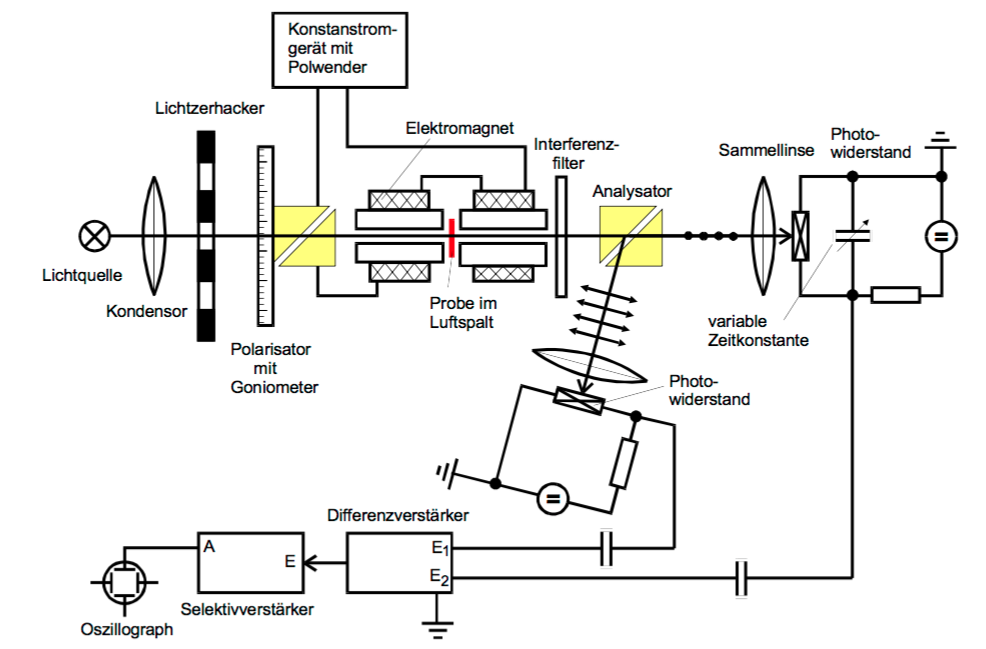
\includegraphics[width=0.9\textwidth]{graphics/setup.png}
    \caption{Schematischer Aufbau des Versuchs \cite{skript}.}
    \label{setup}
\end{figure}
\newpage
\section{Durchführung}
\label{sec:Durchfuehrung}
Es wird das Magnetfeld innerhalb der Spule ausgemessen, um einerseits den Ort des stärksten Feldes und andererseits den Betrag des Magnetfelds zu bestimmen.
Anschließend werden drei Proben,
\begin{itemize}
    \item{GaAs}
    \item{GaAs:Mn (N = \SI{1.2e18}{\per\centi\meter\cubed})}
    \item{GaAs:Mn (N = \SI{2.8e18}{\per\centi\meter\cubed})}
\end{itemize}
bei acht verschiedenen Interferenzfiltern gemessen.
Hierzu wird nach Einsetzen der Probe bei gegebenem Filter das Polarimeter soweit verdreht,
dass das Messsignal Null oder minimal ist. Der Wert des Winkelmessers wird notiert.
Dieser Vorgang wird bei umgepoltem Magnetfeld wiederholt. Da der Faraday-Winkel $\Theta$ linear von dem Magnetfeld abhängt,
ist somit die Differenz der beiden notierten Winkel der doppelten Wert der Faraday-Drehung. Tarieren des Winkelmessers ist nicht erforderlich.
